\documentclass[tikz,border=2mm]{standalone}
\usepackage{pgfplots}
\pgfplotsset{compat=1.17}

\begin{document}

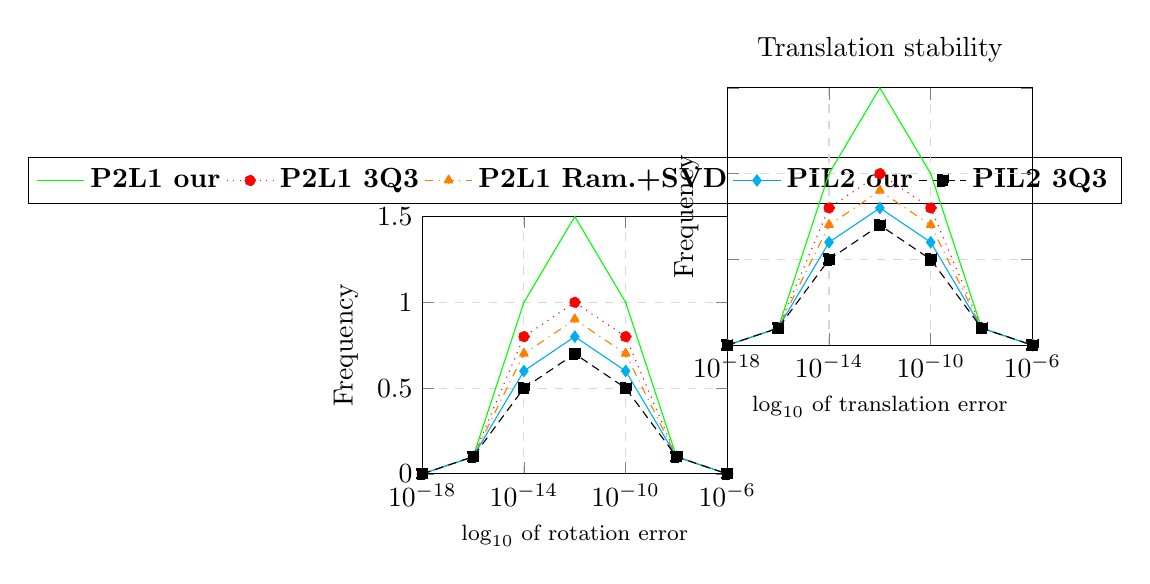
\begin{tikzpicture}
    \begin{axis}[
        name=leftplot,
        width=0.45\textwidth,
        height=0.4\textwidth,
        at={(0,0)},
        xlabel={\footnotesize $\log_{10}$ of rotation error},
        ylabel={Frequency},
        yticklabel style={/pgf/number format/fixed},
        xmode=log,
        xmin=1e-18, xmax=1e-6,
        ymin=0, ymax=1.5,
        title={Rotation stability},
        grid=major,
        grid style={dashed, gray!30},
        legend style={at={(0.5,1.05)}, anchor=south,legend columns=-1},
        cycle list={
            {green,solid},
            {red,dotted},
            {orange,dashdotted},
            {cyan,solid},
            {black,densely dashed},
        }
    ]
        % Example data for demonstration
        \addplot+[mark=none] coordinates {
            (1e-18, 0) (1e-16, 0.1) (1e-14, 1.0) (1e-12, 1.5) (1e-10, 1.0) (1e-8, 0.1) (1e-6, 0)
        };
        \addlegendentry{\textbf{P2L1 our}}
        
        \addplot+[mark=*, red] coordinates {
            (1e-18, 0) (1e-16, 0.1) (1e-14, 0.8) (1e-12, 1.0) (1e-10, 0.8) (1e-8, 0.1) (1e-6, 0)
        };
        \addlegendentry{\textbf{P2L1 3Q3}}
        
        \addplot+[mark=triangle*, orange] coordinates {
            (1e-18, 0) (1e-16, 0.1) (1e-14, 0.7) (1e-12, 0.9) (1e-10, 0.7) (1e-8, 0.1) (1e-6, 0)
        };
        \addlegendentry{\textbf{P2L1 Ram.+SVD}}
        
        \addplot+[mark=diamond*, cyan] coordinates {
            (1e-18, 0) (1e-16, 0.1) (1e-14, 0.6) (1e-12, 0.8) (1e-10, 0.6) (1e-8, 0.1) (1e-6, 0)
        };
        \addlegendentry{\textbf{PIL2 our}}
        
        \addplot+[mark=square*, black] coordinates {
            (1e-18, 0) (1e-16, 0.1) (1e-14, 0.5) (1e-12, 0.7) (1e-10, 0.5) (1e-8, 0.1) (1e-6, 0)
        };
        \addlegendentry{\textbf{PIL2 3Q3}}
    \end{axis}
    
    \begin{axis}[
        name=rightplot,
        width=0.45\textwidth,
        height=0.4\textwidth,
        at={(leftplot.east),xshift=1cm},
        xlabel={\footnotesize $\log_{10}$ of translation error},
        ylabel={Frequency},
        yticklabel style={/pgf/number format/fixed},
        xmode=log,
        xmin=1e-18, xmax=1e-6,
        ymin=0, ymax=1.5,
        title={Translation stability},
        grid=major,
        grid style={dashed, gray!30},
        yticklabels={,,}, % Hide y-axis labels
        legend style={at={(0.5,1.05)}, anchor=south,legend columns=-1},
        cycle list={
            {green,solid},
            {red,dotted},
            {orange,dashdotted},
            {cyan,solid},
            {black,densely dashed},
        }
    ]
        % Example data for demonstration
        \addplot+[mark=none] coordinates {
            (1e-18, 0) (1e-16, 0.1) (1e-14, 1.0) (1e-12, 1.5) (1e-10, 1.0) (1e-8, 0.1) (1e-6, 0)
        };
        
        \addplot+[mark=*, red] coordinates {
            (1e-18, 0) (1e-16, 0.1) (1e-14, 0.8) (1e-12, 1.0) (1e-10, 0.8) (1e-8, 0.1) (1e-6, 0)
        };
        
        \addplot+[mark=triangle*, orange] coordinates {
            (1e-18, 0) (1e-16, 0.1) (1e-14, 0.7) (1e-12, 0.9) (1e-10, 0.7) (1e-8, 0.1) (1e-6, 0)
        };
        
        \addplot+[mark=diamond*, cyan] coordinates {
            (1e-18, 0) (1e-16, 0.1) (1e-14, 0.6) (1e-12, 0.8) (1e-10, 0.6) (1e-8, 0.1) (1e-6, 0)
        };
        
        \addplot+[mark=square*, black] coordinates {
            (1e-18, 0) (1e-16, 0.1) (1e-14, 0.5) (1e-12, 0.7) (1e-10, 0.5) (1e-8, 0.1) (1e-6, 0)
        };
    \end{axis}
\end{tikzpicture}

\end{document}